\chapter{ATMega32u4}

\section{Register beschreiben}
Ein Bit in einem Register kann entweder auf \verb|0| oder \verb|1| gesetzt werden. \\
Um es auf \verb|0| zu setzen, muss es mit \verb|0| ge-UND-et werden und wird mit dem Zeichen \verb|&| dargestellt. \\

Der Code, um das \textbf{4. Bit} (es wird bei \verb|0| angefangen zu zählen), auf \verb|0| zu setzen, sieht folgendermaßen aus:
\begin{lstlisting}[language=C]
// REGISTER = REGISTER &~ (0 << POSITION IM REGISTER)
DDRD = DDRD &~ (1 << 3);
\end{lstlisting}
Die Tilde (\verb|~|) ist hier ein Negator, d.h. es ist \textbf{nicht} 1, also 0; die Pfeile sind Shiebeoperatoren, um das korrekte Bit anzusprechen.
\vspace{0.5cm}

Ähnlich ist es beim Setzen eines Bits auf \verb|1|: Hier wird mit \verb|1| ge-ODER-et, was mit dem Zeichen \verb$|$ gezeigt wird:
\begin{lstlisting}[language=C]
// REGISTER = REGISTER | (1 << POSITION IM REGISTER)
DDRD = DDRD | (1 << 3);
\end{lstlisting}

\vspace{0.5cm}

Es können jeweils \textbf{mehrere} Bits eines Registers in einer Zeile auf 1 \textbf{oder} 0 gesetzt werden. Allerdings darf in einer Zeile ein Bit nicht auf 0, während ein anderes auf 1 gesetzt werden.

\begin{itemize}
    \item \underline{Erlaubt:} \\
    \verb|DDRD = DDRD &~ (1 << 3) &~ (1 << 3) &~ (1 << 3);|
    \item \underline{Nicht erlaubt:} \\
    \verb$DDRD = DDRD | (1 << 3) | (1 << 3) &~ (1 << 3);$
\end{itemize}

\newpage

\section{Takt}
Der Takt des ATMega32u4 kann per Software verringert werden und wird über das \verb|CLKPR|-Register getan. Bevor dieses beschrieben werden kann, muss \verb|0x80| in das Register geschrieben werden.

\vspace{0.5cm}
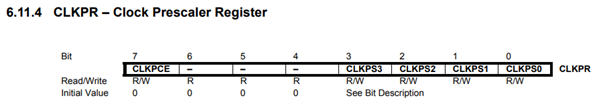
\includegraphics{Atmega/CLKPR.png}

\vspace{0.5cm}
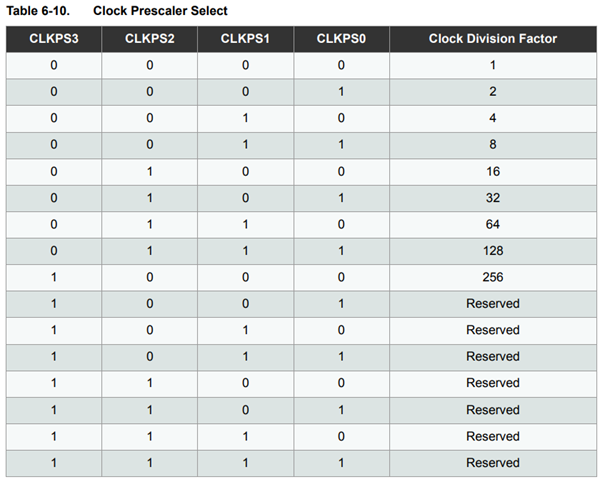
\includegraphics{Atmega/CLKPR-Table.png}

\newpage

\subsubsection*{Beispiel}
Der externe Takt hat 16MHz und soll auf 8MHz heruntergesetzt werden.
\begin{lstlisting}[language=C]
    CLKPR = 0x80;
    CLKPR = 0x01;
\end{lstlisting}

\section{GPIO}
Die \textbf{General-Purpose-Input-Output}-Pins (GPIO-Pins) können folgenden Status haben:
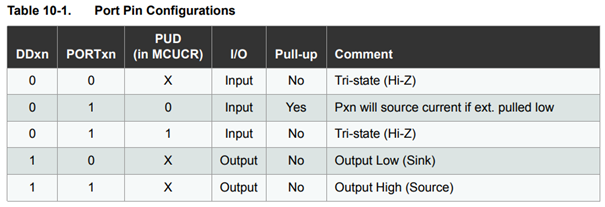
\includegraphics{Atmega/PortPin-Config.png}

\subsubsection*{Beispiel}
Pin-D7 auf HIGH setzen.
\begin{lstlisting}[language=C]
    DDRD = DDRD | (1 << DDD7);
    PORTD = PORTD | (1 << PORTD7);
\end{lstlisting}

\vspace{1cm}

\textbf{Wichtig:} Bei der Verwendung von Hardwareeinheiten (Timer, UART, etc.) muss GPIO immer \underline{zuerst} auf Input bzw. Output eingestellt werden.

\newpage

\section{ADC}
\begin{itemize}
    \item \underline{Single-Ended:} \\
    Spannung von ADC-Pin zu GND wird gemessen.
    \item \underline{Differenziell:} \\
    Spannung zwischen zwei ADC-Pins wird gemessen. (Siehe Kapitel \ref{})
    \item \underline{Referenzspannung:} \\
    Es gibt drei verschiedene Spannungsreferenzen:
    \begin{itemize}
        \item Interne 2,56V Referenz
        \item Externer \verb|AREF|-Pin
        \item Externer \verb|AVCC|-Pin
    \end{itemize}
    \item \underline{Auto-Trigger Mode} \\
    Es wird periodisch gemessen, wofür die Taktquelle eingestellt werden muss. (Siehe Kapitel \ref{Atmega/AutoTrigger})
\end{itemize}

\subsection{Differenziell} \label{Atmega/Differenziell}
Wenn differenziell gemessen wird, ist das Ergebnis im Zweierkomplement dargestellt - ein Zahlensystem um negative Zahlen (in binär) darzustellen.
\subsubsection*{Beispiel}
"$-2_d$" im Zweierkomplement \\
\begin{enumerate}
    \item Zunächst wird der Binärwert des Betrags der Zahl invertiert: $2_d=0010_b\Rightarrow 1101_b$ \\
    \item Danach wird zu diesem Wert $1_b$ addiert: $1101_b + 1_b = 1110_b = -2_d$
\end{enumerate}

\newpage

\subsection{Auto-Trigger Mode} \label{Atmega/AutoTrigger}
Die Taktquelle wird folgendermaßen eingestellt:

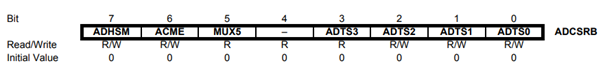
\includegraphics{Atmega/AutoTrigger-Reg.png}
\vspace{0.5cm}
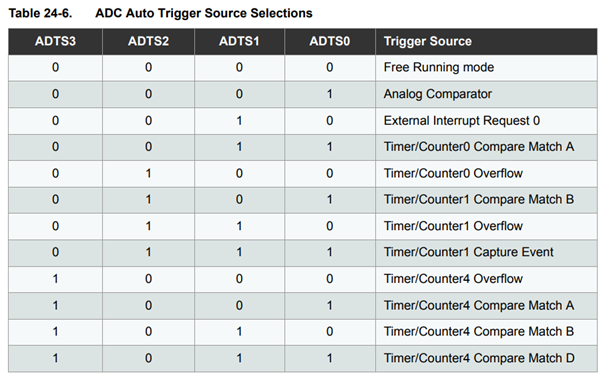
\includegraphics{Atmega/ADC-AutoTrigger-Select.png}

\subsubsection*{Ergebnis}
Das Messergebnis des ADC befindet sich in zwei Registern: \verb|ADCL| (ADC-Low) und \verb|ADCH| (ADC-High).

\newpage

Der Messwert kann in zwei Arten dargestellt werden:
\begin{enumerate}
    \item \underline{Linksbündig:} \\
    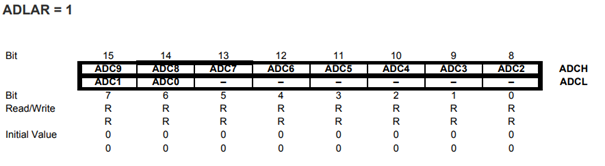
\includegraphics{Atmega/ADLAR-1.png}
    \item \underline{Rechtsbündig:} \\
    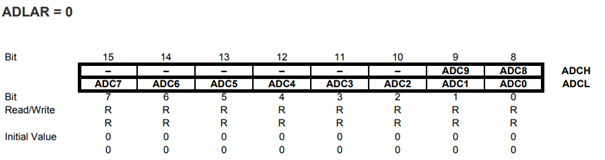
\includegraphics{Atmega/ADLAR-0.png}
\end{enumerate}

\verb|ADCL| muss immer vor \verb|ADCH| ausgelesen werden; folgende Beispiele verwenden Linksbündigkeit.\\

\newpage

\subsection{Messdauer berechnen}
Die ADC Messdauer muss eingestellt werden: kurze Messdauern führen zu ungenaueren Erbenissen, bei zu langen kann die Dauer zwischen Abtastpunkten zu groß werden. Generell sollte die Messfrequenz des ATMega32u4 zwischen $50kHz$ und $200kHz$ sein (wenn die Messgeschwindigkeit realisierbar ist.)

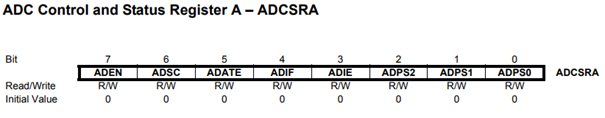
\includegraphics{Atmega/ADC-Control-Status.png}
\vspace{0.5cm}
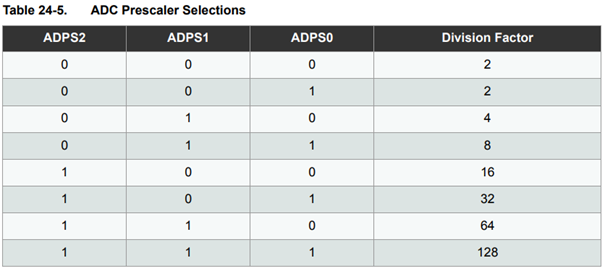
\includegraphics{Atmega/ADC-Prescaler.png}

Der Wert des obigen Diagramms muss in die gemessene Spannung umgerechnet werden.
\begin{itemize}
    \item \underline{Single-Ended}:
    \begin{align}
        V_{IN} = \frac{ADC \cdot V_{REF}}{1023}
    \end{align}
    \item \underline{Differenziell}:\\
    \begin{align}
        V_{POS} - V_{NEG} = \frac{ADC \cdot V_{REF}}{GAIN \cdot 512}
    \end{align}
\end{itemize}

\newpage

\subsubsection*{Single-Ended}
Der entsprechende Code um die gemessene Spannung zurückzubekommen:
\begin{lstlisting}[language=C]
// SETUP:
DDRF = DDRF &~ (1 << DDF0);	 // PF0-Input
ADMUX = ADMUX | (1 << ADLAR) | (1 << REFS0); // Left adjust ADC result; Voltage reference

// Uncomment for Auto trigger mode; 
// ADCSRA = ADCSRA | (1 << ADATE);
// ADCSRB = ADCSRB | (1 << ADTS1) | (1 << ADTS0); // Auto trigger mode Taktquelle (Timer0)

// Enable Interrupt
// Enable ADC
// Prescaler = 64: ADC_f = 8M/64
ADCSRA = ADCSRA | (1 << ADEN) | (1 << ADSC) | (1 << ADPS2) | (1 << ADPS1);
DIDR0 = DIDR0 | (1 << ADC0D); // Disable digital function of PF0

// READ:
adcRead() {
    uint16_t adc_value;
    float out;
    unsigned char adcl, adch;

    // Start conversation
    // Put in comment in auto trigger mode
    ADCSRA = ADCSRA | (1 << ADSC);

    // Wait for ADC to finish
    while(ADCSRA & (1 << ADSC))  {}

    adcl = ADCL;
    adch = ADCH;
    adc_value = (adcl >> 6) + (adch << 2);
    out = (float)((adc_value * 5) / 1023.0);
    return out;
}
\end{lstlisting}
\todo{No return type?}

\subsubsection*{Differenziell}
Auch hier der Code, um die Spannung returniert zu bekommen:
\begin{lstlisting}[language=C]
// SETUP:
DDRF = DDRF &~ (1 << DDF0) &~ (1 << DDF1); // PF0-Input
ADMUX = ADMUX | (1 << ADLAR) | (1 << REFS0); // Left adjust ADC result; Voltage reference
ADMUX = ADMUX | (1 << MUX4); // PINS(P:ADC0; N: ADC1); GAIN: 1

// Uncomment for auto trigger mode
// ADCSRA = ADCSRA | (1 << ADATE);	
// ADCSRB = ADCSRB | (1 << ADTS1) | (1 << ADTS0); // Auto trigger mode Taktquelle (Timer0)

// Enable interrupt enable
// Enable ADC
// Prescaler = 64: ADC_f = 8M/64
ADCSRA = ADCSRA | (1 << ADEN) | (1 << ADSC) | (1 << ADPS2) | (1 << ADPS1);
    
// READ:
adcRead() {
    uint16_t adc_value;
    float out;
    unsigned char adcl, adch;
    
    // Start conversation
    // Put in comment in auto trigger mode
    ADCSRA = ADCSRA | (1 << ADSC);

    // Wait for ADC to finish
    while(ADCSRA & (1 << ADSC)) {}
    adcl = ADCL;
    adch = ADCH;
    adc_value = (adcl >> 6) + (adch << 2);
    out = (float)((adc_value * 5) / (1.0 * 1023.0));
    return out;
}
\end{lstlisting}

\section{Sleep Mode}
\subsubsection*{Idle Mode}
Der CPU- und Flash-Clock wird gestoppt, alle anderen Clocks laufen weiter. Jedoch funktionieren Peripherien, wie: Timer, USB, SPI, USART, ADC, Analog-Komperator, I2C Watchdog, Interrupts. \\
Der Mikrocontroller kann durch interne und externe Interrupts - z.B. Timer-Overflow, USART, Transmition-Complete, etc. - aufgeweckt werden.

\subsubsection*{ADC Noise Reduction Mode}
Dieser Modus ist dafür da, um die Genauigkeit der ADC-Messungen zu erhöhen. Wenn der ADC aktiviert ist, und dieser Noise Reduction Mode ebenso, startet automatisch eine ADC-Messung. \\
Alles bis auf ADC, externe Interrupts, I2C-Address-Matching und den Watchdog-Timer wird abgeschaltet. \\

Der Mikrocontroller kann durch die Vollendung der ADC-MEssung, Reset, Watchdog-Timer, Brownout-Reset, I2C-Interrupt, SPM/EEPROM-Interrupt und externe Interrupts - an den Pins \verb|INT3:0|, \verb|INT6| - oder Pin-Change-Interrupts aufgeweckt werden.

\subsubsection*{Power-Down/-Save Mode}
Der externe Clock wird deaktiviert, wodurch asynchrone Peripherien - externe Interrupts, I2C-Interrupt, Watchdog - weiterarbeiten. \\

Der Controller kann durch Reset, Watchdog, Brownout-Reset, I2C-Address-Match und externe Interrupts (an den Pins \verb|INT3:0|, \verb|INT6|) Pin-Change-Interrupts aufgeweckt werden. \\

Merke, dass dieser Modus mehr Zeit benötigt, um wieder aufzuwachen.

\subsubsection*{(Extended) Standby Mode}
Dieser Modues ist im Endeffekt gleich wie der Power-Down Mode, nur hier ist der verwendete Oszillator nicht gestoppt wird; dadurch erwacht der Mikrocontroller schneller.

\subsubsection*{Register}
Um die Sleep-Modi zu aktivieren, muss die \verb|avr/sleep.h|-Library inkludiert werden. \\
Zunächst muss eingestellt werden, wie der Controller aufgeweckt wird. Eine einfache Methode dafür ist der Watchdog-Timer, der, sobald er aktiviert wurde, immer im Hintergrund läuft. Um die Bits \verb|WDE| oder \verb|WDPx| des Watchdog-Registers \verb|WDTCSR| verändern zu können, muss gleichzeitig auch das \verb|WDCE|-Bit gesetzt werden. \\
(Dieses Bit wird automatisch zurückgesetzt.) \\

Mit dem \verb|WDIE|-Bit des \verb|WDTCSR|-Registers, wird der Interrupt, welcher den Mikrocontroller aufweckt, aktiviert. \\

Mit den Bits \verb|WDP0| bis \verb|WDP3| wird die Sleep-Zeit eingestellt. \\

Mit der Funktion \verb|set_sleep_mode(MODE);| wird der Sleep-Mode eingestellt. Folgendes kann für \verb|MODE| eingesetzt werden:
\begin{itemize}
    \item \verb|SLEEP_MODE_IDLE|
    \item \verb|SLEEP_MODE_PWR_DOWN|
    \item \verb|SLEEP_MODE_PWR_SAVE|
    \item \verb|SLEEP_MODE_ADC|
    \item \verb|SLEEP_MODE_STANDBY|
    \item \verb|SLEEP_MODE_EXT_STANDBY|
\end{itemize}

Mit der Funktion \verb|sleep_mode();| wird der Sleep-Mode aktiviert. \\

\subsubsection*{Beispiel}
\begin{lstlisting}[language=C]
#include <avr/io.h>
#include <util/delay.h>
#include <avr/interrupt.h>
#include <avr/sleep.h>

int main(void) {
    DDRB = 255;

    WDTCSR = 0b01010100;
    WDTCSR = 0b01010100; // Sicherheitshalber 2-mal schreiben

    // Global ISR (Interrupt Service Routine) aktivieren
    sei(); 

    set_sleep_mode(SLEEP_MODE_PWR_DOWN); // Sleep-Mode setzen

    while(1) {
	    PORB ^= PORTB;
        sleep_mode();
    }
}
\end{lstlisting}

\section{Power Saving}
\subsection{Peripherien}
Mit Hilfe der Power-Reduction-Register \verb|PRR0| und \verb|PRR1| kann der Clock zu einzelnen Peripherien ausgeschaltet werden. Diese werden "eingefroren"; sobald sie wieder aktiviert werden, arbeiten sie dort weiter, wo sie aufgehört haben.\\
Merke, dass einige der Bit-Namen des \verb|PRR1|-Registers nicht richtig hinterlegt sind und deswegen Compilefehler auftauchen können.
\subsection{Pins}
Weiterhin sollten alle nicht verwendeten Pins auf Input-mit-Pullup geschalten werden, d.h. im Programm:
\begin{lstlisting}[language=C]
    DDRx = 0;
    PORTx = 255;
\end{lstlisting}
Weil diese Pins jetzt keine Outputs mehr sind, geht kein Strom "verloren". Sie als Input-\underline{Pullup} zu definieren, verhindert, dass die CMOS-Eingänge ununterbrochen schalten (das auch zu Verlusten führen würde).

\section{Externe Interrupts}
Externe Interrupts lösen eine Funktion aus, wenn eine Zustandsänderung an einem Pin eintritt. Dieser Pin muss zuvor richtig als Eingang \todo {und Ausgang?} definiert werden. Außerdem müssen Interrupts global mittels \verb|sei();| aktiviert sein. \\

Es gibt zwei verschiedene Arten von externen Interrupts:
\begin{enumerate}
    \item \underline{"Normale" Interrupts} \\
    Hier wird ein Pin einzel betrachtet; mit dem \verb|EICRA|- bzw. \verb|EICRB|-Regsiter wird die Flanke, auf die geachtet werden soll, eingestellt. \\
    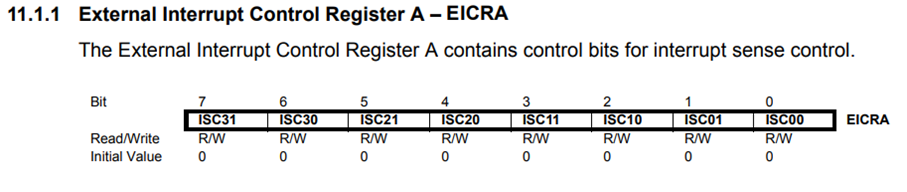
\includegraphics{Atmega/EICRA-Reg.png}
    \vspace{0.5cm}
    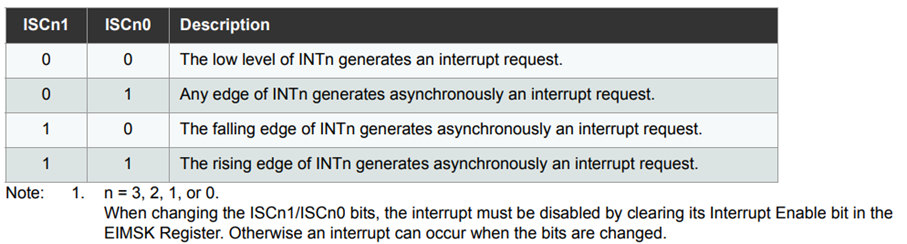
\includegraphics{Atmega/EICRA-Description.png}
    Mit dem \verb|EIMSK|-Register werden die einzelnen Pin-Interrupts freigegeben. \\
    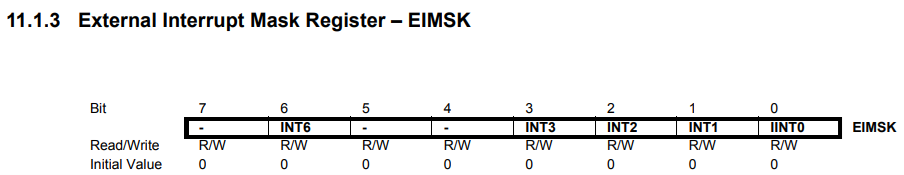
\includegraphics{Atmega/EIMSK-Table.png}

    \item \underline{Pin-Change Interrupts} \\
    Alle Pins des \verb$B$-Registers können einen gemeinsamen Interrupt auslösen - egal auf welchem Pin die Zustandsänderung auftritt, es wird derselbe Interrupt ausgelöst. \\
    Die Flanke, auf die geachtet wird, kann nicht eingestellt werden; es wird auf eine beliebige Flankenänderung gewartet.\\

    Mit dem \verb|PCICR|-Register wird der Pin-Change Interrupt aktiviert. \\
    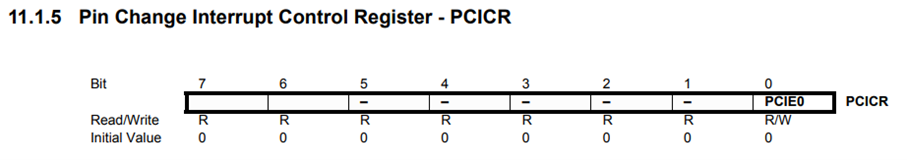
\includegraphics{Atmega/PCICR-Reg.png}
    \vspace{0.5cm}
    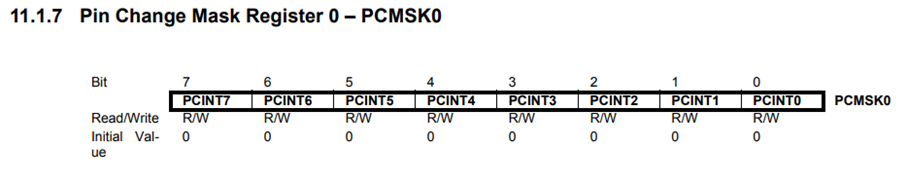
\includegraphics{Atmega/PCMSK0-Reg.png}
\end{enumerate}